
%% Magnetism Questions used on the
%% NYSED Physics Regents Examination
%%--------------------------------------------------

%% this section contains 30 problems


%% Section June2014
%%--------------------
\element{nysed}{
\begin{question}{June2014-Q11}
    An electron moving at constant speed produces:
    \begin{choices}
      \correctchoice{both a magnetic and an electric field}
        \wrongchoice{an electric field, only}
        \wrongchoice{a magnetic field, only}
        \wrongchoice{neither a magnetic nor an electric field}
    \end{choices}
\end{question}
}

%% Section June2013
%%--------------------
\element{nysed}{
\begin{question}{June2013-Q28}
    Which particle would produce a magnetic field?
    \begin{choices}
        \wrongchoice{a neutral particle moving in a straight line}
        \wrongchoice{a neutral particle moving in a circle}
        \wrongchoice{a stationary charged particle}
      \correctchoice{a moving charged particle}
    \end{choices}
\end{question}
}


%% Section June2012
%%--------------------
\element{nysed}{
\begin{question}{June2012-Q30}
    A small object is dropped through a loop of wire connected to a sensitive ammeter on the edge of a table,
        as shown in the diagram below.
    \begin{center}
        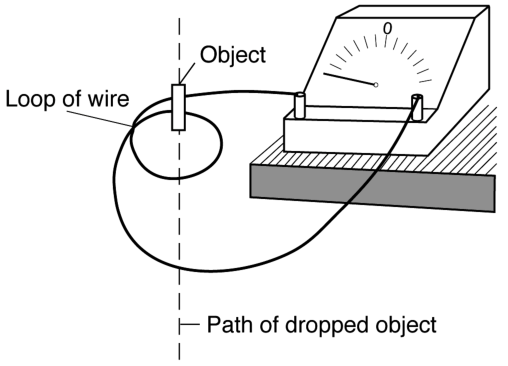
\includegraphics[keepaspectratio,scale=0.75]{June2012-Q30}
    \end{center}
    A reading on the ammeter is most likely produced when the object falling through the loop of wire is a:
    \begin{multicols}{2}
    \begin{choices}
        \wrongchoice{flashlight battery}
      \correctchoice{bar magnet}
        \wrongchoice{brass mass}
        \wrongchoice{plastic ruler}
    \end{choices}
    \end{multicols}
\end{question}
}


%% Section June2011
%%--------------------
\element{nysed}{
\begin{question}{June2011-Q24}
    Moving a length of copper wire through a magnetic field may cause the wire to have a:
    \begin{choices}
      \correctchoice{potential difference across it}
        \wrongchoice{lower temperature}
        \wrongchoice{lower resistivity}
        \wrongchoice{higher resistance}
    \end{choices}
\end{question}
}

\element{nysed}{
\begin{question}{June2011-Q45}
    The diagram below shows the magnetic field lines between two magnetic poles, $A$ and $B$.
    \begin{center}
    \begin{tikzpicture}
        %% magnet A
        \draw[thick] (-3.5,-0.5) rectangle (-1,0.5);
        \node[anchor=east] at (-1,0) {$A$};
        \node[anchor=west] at (-3.5,0) {Magnet};
        %% magnet B
        \draw[thick] (+3.5,-0.5) rectangle (+1,0.5);
        \node[anchor=west] at (+1,0) {$B$};
        \node[anchor=east] at (+3.5,0) {Magnet};
        %% field lines
        \begin{scope}[decoration={markings,mark=at position 0.5 with {\arrow{latex}}}]
            \draw[thick,postaction={decorate}] (-1,0.5) to [out=15,in=165] (+1,0.5);
            \draw[thick,postaction={decorate}] (-1,0.25) to [out=5,in=175] (+1,0.25);
            \draw[thick,postaction={decorate}] (-1,0.0) to [out=0,in=180] (+1,0.0);
            \draw[thick,postaction={decorate}] (-1,-0.25) to [out=355,in=185] (+1,-0.25);
            \draw[thick,postaction={decorate}] (-1,-0.5) to [out=345,in=195] (+1,-0.5);
        \end{scope}
    \end{tikzpicture}
    \end{center}
    Which statement describes the polarity of magnetic poles $A$ and $B$?
    \begin{choices}
      \correctchoice{$A$ is a north pole and $B$ is a south pole.}
        \wrongchoice{$A$ is a south pole and $B$ is a north pole.}
        \wrongchoice{Both $A$ and $B$ are north poles.}
        \wrongchoice{Both $A$ and $B$ are south poles.}
    \end{choices}
\end{question}
}

%% Section June2010
%%--------------------
\element{nysed}{
\begin{question}{June2010-Q19}
    Magnetic fields are produced by particles that are:
    \begin{choices}
      \correctchoice{moving and charged}
        \wrongchoice{moving and neutral}
        \wrongchoice{stationary and charged}
        \wrongchoice{stationary and neutral}
    \end{choices}
\end{question}
}


%% Section June2009
%%--------------------
\element{nysed}{
\begin{question}{June2009-Q22}
    When two ring magnets are placed on a pencil,
        magnet $A$ remains suspended above magnet $B$, as shown below.
    \begin{center}
        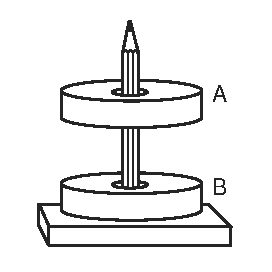
\includegraphics[keepaspectratio,scale=0.75]{June2009-Q22}
    \end{center}
    Which statement describes the gravitational force and the magnetic force acting on magnet $A$ due to magnet $B$?
    \begin{choices}
      \correctchoice{The gravitational force is attractive and the magnetic force is repulsive.}
        \wrongchoice{The gravitational force is repulsive and the magnetic force is attractive.}
        \wrongchoice{Both the gravitational force and the magnetic force are attractive.}
        \wrongchoice{Both the gravitational force and the magnetic force are repulsive.}
    \end{choices}
\end{question}
}


%% Section Jan2009
%%--------------------
\element{nysed}{
\begin{question}{Jan2009-Q21}
    The diagram below represents a \SI{0.5}{\kilo\gram} bar magnet and a \SI{0.7}{\kilo\gram} bar magnet with a distance of \SI{0.2}{\meter} between their centers.
    \begin{center}
    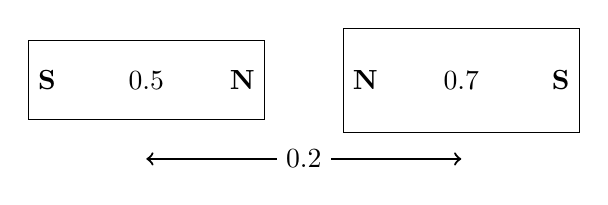
\begin{tikzpicture}
        \begin{scope}[xshift=-2cm]
            \draw (-1.5,-0.5) rectangle (1.5,0.5);
            \node[anchor=center] at (0,0) {\SI{0.5}{\kilo\gram}};
            \node[anchor=west] at (-1.5,0) {\bfseries S};
            \node[anchor=east] at (+1.5,0) {\bfseries N};
        \end{scope}
        \begin{scope}[xshift=+2cm]
            \draw (-1.5,-0.66) rectangle (1.5,0.66);
            \node[anchor=center] at (0,0) {\SI{0.7}{\kilo\gram}};
            \node[anchor=west] at (-1.5,0) {\bfseries N};
            \node[anchor=east] at (+1.5,0) {\bfseries S};
        \end{scope}
        \draw[thick,<->] (-2,-1) -- (2,-1) node[pos=0.5,anchor=center,fill=white] {\SI{0.2}{\meter}};
    \end{tikzpicture}
    \end{center}
    Which statement best describes the forces between the bar magnets?
    \begin{choices}
        \wrongchoice{Gravitational force and magnetic force are both repulsive.}
        \wrongchoice{Gravitational force is repulsive and magnetic force is attractive.}
      \correctchoice{Gravitational force is attractive and magnetic force is repulsive.}
        \wrongchoice{Gravitational force and magnetic force are both attractive.}
    \end{choices}
\end{question}
}


%% Section June2008
%%--------------------


%% Section Jan2008
%%--------------------


%% Section June2007
%%--------------------
\element{nysed}{
\begin{question}{June2007-Q01}
    Which is \emph{not} a vector quantity?
    \begin{choices}
      \correctchoice{electric charge}
        \wrongchoice{magnetic field strength}
        \wrongchoice{velocity}
        \wrongchoice{displacement}
    \end{choices}
\end{question}
}


%% Section Jan2007
%%--------------------


%% Section June2006
%%--------------------


%% Section Jan2006
%%--------------------
\element{nysed}{
\begin{question}{Jan2006-Q39}
    An electrical generator in a science classroom makes a lightbulb glow when a student turns a hand crank on the generator.
    During its operation, this generator converts:
    \begin{choices}
        \wrongchoice{chemical energy to electrical energy}
      \correctchoice{mechanical energy to electrical energy}
        \wrongchoice{electrical energy to mechanical energy}
        \wrongchoice{electrical energy to chemical energy}
    \end{choices}
\end{question}
}


%% Section June2005
%%--------------------
\element{nysed}{
\begin{question}{June2005-Q15}
    The diagram below shows the lines of magnetic force between two north magnetic poles.
    \begin{center}
    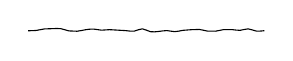
\begin{tikzpicture}
        %% NOTE: TODO: draw tikz
        %% left magnet
        \draw plot [smooth,tension=0.7,samples=30,domain={-1.5:1.5}] (\x,3 + 0.02*rand);
        %% right magnet
    \end{tikzpicture}
    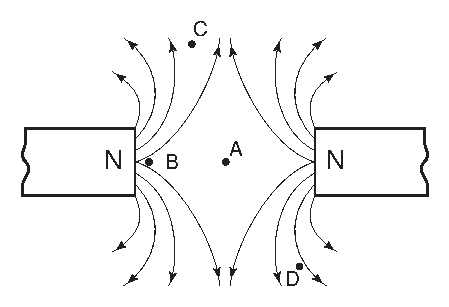
\includegraphics[keepaspectratio,scale=0.75]{June2005-Q15}
    \end{center}
    At which point is the magnetic field strength greatest?
    \begin{multicols}{4}
    \begin{choices}[o]
        \wrongchoice{$A$}
      \correctchoice{$B$}
        \wrongchoice{$C$}
        \wrongchoice{$D$}
    \end{choices}
    \end{multicols}
\end{question}
}


%% Section Jan2005
%%--------------------


%% Section June2004
%%--------------------
\element{nysed}{
\begin{question}{June2004-Q16}
    Which type of field is present near a moving electric charge?
    \begin{choices}
        \wrongchoice{an electric field, only}
        \wrongchoice{a magnetic field, only}
      \correctchoice{both an electric field and a magnetic field}
        \wrongchoice{neither an electric field nor a magnetic field}
    \end{choices}
\end{question}
}

\element{nysed}{
\begin{question}{June2004-Q25}
    The energy equivalent of the rest mass of an electron is approximately:
    \begin{multicols}{2}
    \begin{choices}
        \wrongchoice{\SI{5.1e5}{\joule}}
      \correctchoice{\SI{8.2e-14}{\joule}}
        \wrongchoice{\SI{2.7e-22}{\joule}}
        \wrongchoice{\SI{8.5e-28}{\joule}}
    \end{choices}
    \end{multicols}
\end{question}
}


%% Section Jan2004
%%--------------------
\element{nysed}{
\begin{question}{Jan2004-Q20}
    In order to produce a magnetic field,
        an electric charge must be
    \begin{multicols}{2}
    \begin{choices}
        \wrongchoice{stationary}
      \correctchoice{moving}
        \wrongchoice{positive}
        \wrongchoice{negative}
    \end{choices}
    \end{multicols}
\end{question}
}


%% Section June2003
%%--------------------
\element{nysed}{
\begin{question}{June2003-Q14}
    The diagram below represents the magnetic field near point $P$.
    \begin{center}
    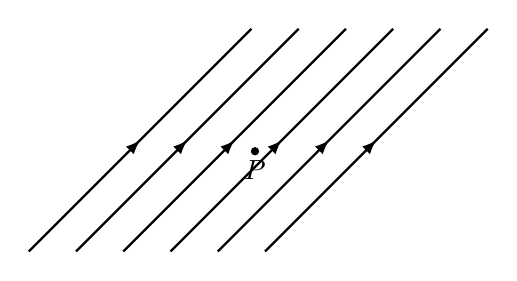
\begin{tikzpicture}
        %% field lines
        \foreach \x in {0,6,...,32}
            \draw[thick,-latex] (\x mm,0) -- ++(45:-4) -- ++(45:2);
        %% point P
        \fill (16 mm,0) ++ (45:-2.2) circle (1.5pt) node[anchor=north] {$P$};
    \end{tikzpicture}
    \end{center}
    If a compass is placed at point $P$ in the same plane as the magnetic field,
        which arrow represents the direction the north end of the compass needle will point?
    \begin{multicols}{2}
    \begin{choices}
        \AMCboxDimensions{down=-0.4cm}
        \wrongchoice{
            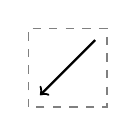
\begin{tikzpicture}
                \draw[dashed,white!50!black] (0,0) rectangle (1,1);
                \draw[thick,->] (0.85,0.85) -- (0.15,0.15);
            \end{tikzpicture}
        }
        %% North will point in the direction of the B field
        \correctchoice{
            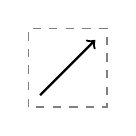
\begin{tikzpicture}
                \draw[dashed,white!50!black] (0,0) rectangle (1,1);
                \draw[thick,->] (0.15,0.15) -- (0.85,0.85);
            \end{tikzpicture}
        }
        \wrongchoice{
            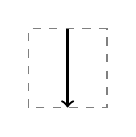
\begin{tikzpicture}
                \draw[dashed,white!50!black] (0,0) rectangle (1,1);
                \draw[thick,->] (0.5,1) -- (0.5,0);
            \end{tikzpicture}
        }
        \wrongchoice{
            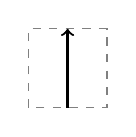
\begin{tikzpicture}
                \draw[dashed,white!50!black] (0,0) rectangle (1,1);
                \draw[thick,->] (0.5,0) -- (0.5,1);
            \end{tikzpicture}
        }
    \end{choices}
    \end{multicols}
\end{question}
}

\element{nysed}{
\begin{question}{June2003-Q22}
    The diagram below shows a wire moving to the right at speed $v$ through a uniform magnetic field that is directed into the page.
    \begin{center}
    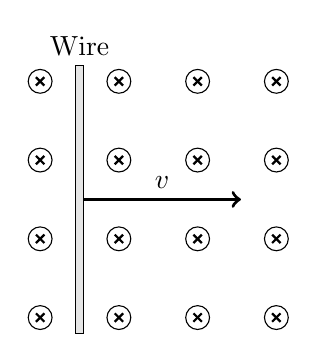
\begin{tikzpicture}
        %% B field into page
        \foreach \x in {0,1,2,3}
            \foreach \y in {0,1,2,3} {
                \draw (\x,\y) circle (1ex);
                \foreach \z in {45,135,225,315} {
                    \draw[thick] (\x,\y) -- ++(\z:-0.5ex);
                } 
            }
        %% wire
        \draw[fill=white!90!black] (0.45,3.2) rectangle (0.55,-0.2);
        \draw[very thick,->] (0.55,1.5) -- ++(0:2) node[pos=0.5,anchor=south] {$v$};
        \node[anchor=south] at (0.5,3.2) {Wire};
    \end{tikzpicture}
    \end{center}
    As the speed of the wire is increased,
        the induced potential difference will:
    \begin{choices}
        \wrongchoice{decrease}
      \correctchoice{increase}
        \wrongchoice{remain the same}
    \end{choices}
\end{question}
}



%% Section Jan2003
%%--------------------
\element{nysed}{
\begin{question}{Jan2003-Q44}
    The diagram below shows a bar magnet.
    \begin{center}
    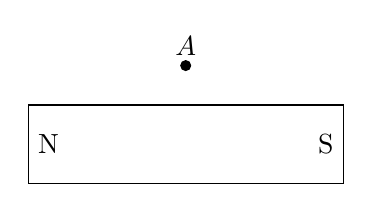
\begin{tikzpicture}
        \draw (-2,-0.5) rectangle (2,0.5);
        \node[anchor=west] at (-2,0) {N};
        \node[anchor=east] at (+2,0) {S};
        \fill (0,1) circle (2pt) node[anchor=south] {$A$};
    \end{tikzpicture}
    \end{center}
    Which arrow best represents the direction of the
        needle of a compass placed at point $A$?
    \begin{multicols}{2}
    \begin{choices}
        \AMCboxDimensions{down=-0.8cm}
        \wrongchoice{
            \begin{tikzpicture}[scale=2]
                \draw[dashed,white!60!black] (0,0) rectangle (1,1);
                \draw[thick,->] (0.5,0) -- (0.5,1);
            \end{tikzpicture}
        }
        \wrongchoice{
            \begin{tikzpicture}[scale=2]
                \draw[dashed,white!60!black] (0,0) rectangle (1,1);
                \draw[thick,->] (0.5,0) -- (0.5,1);
            \end{tikzpicture}
        }
        \correctchoice{
            \begin{tikzpicture}[scale=2]
                \draw[dashed,white!60!black] (0,0) rectangle (1,1);
                \draw[thick,->] (0,0.5) -- (1,0.5);
            \end{tikzpicture}
        }
        \wrongchoice{
            \begin{tikzpicture}[scale=2]
                \draw[dashed,white!60!black] (0,0) rectangle (1,1);
                \draw[thick,->] (1,0.5) -- (0,0.5);
            \end{tikzpicture}
        }
    \end{choices}
    \end{multicols}
\end{question}
}


%% Section Aug2002
%%--------------------
\element{nysed}{
\begin{question}{Aug2002-Q30}
    Which diagram best represents magnetic flux lines around a bar magnet?
    \begin{multicols}{2}
    \begin{choices}[o]
        \AMCboxDimensions{down=-1.2cm}
        \wrongchoice{
            \begin{tikzpicture}
            \draw[dashed,white!60!black] (-1.5,-1.5) rectangle (+1.5,1.5);
            \clip (-1.5,-1.5) rectangle (+1.5,1.5);
            \begin{scope}[decoration={markings,mark=at position 0.05 with {\arrow{latex}}}]
                %% magnet
                \draw (-1,-0.25) rectangle (1,0.25);
                \node[anchor=west] at (-1,0) {N};
                \node[anchor=east] at (+1,0) {S};
                %% field lines
                %\draw[thick,-latex] (-1,-0.1) arc();
                %\draw[thick,-latex] (-1,+0.1) .. controls ++(225:5) and ++(315:5) .. (1,+0.1);
            \end{scope}
            \end{tikzpicture}
        }
        \wrongchoice{
            \begin{tikzpicture}
            \draw[dashed,white!60!black] (-1.5,-1.5) rectangle (+1.5,1.5);
            \clip (-1.5,-1.5) rectangle (+1.5,1.5);
            \begin{scope}[decoration={markings,mark=at position 0.5 with {\arrow{latex}}}]
                %% magnet
                \draw (-1,-0.25) rectangle (1,0.25);
                \node[anchor=west] at (-1,0) {N};
                \node[anchor=east] at (+1,0) {S};
                %% field lines
                \draw[thick,postaction={decorate}] (-1,-0.12) .. controls ++(135:2) and ++(45:2) .. (1,-0.12);
                \draw[thick,postaction={decorate}] (-1,+0.12) .. controls ++(225:2) and ++(315:2) .. (1,+0.12);
            \end{scope}
            \end{tikzpicture}
        }
        \correctchoice{
            \begin{tikzpicture}
            \draw[dashed,white!60!black] (-1.5,-1.5) rectangle (+1.5,1.5);
            \clip (-1.5,-1.5) rectangle (+1.5,1.5);
            \begin{scope}[decoration={markings,mark=at position 0.5 with {\arrow{latex}}}]
                %% magnet
                \draw (-1,-0.25) rectangle (1,0.25);
                \node[anchor=west] at (-1,0) {N};
                \node[anchor=east] at (+1,0) {S};
                %% field lines
                \draw[thick,postaction={decorate}] (-1,+0.1) .. controls ++(135:1.25) and ++(45:1.25) .. (1,+0.1);
                \draw[thick,postaction={decorate}] (-1,-0.1) .. controls ++(225:1.25) and ++(315:1.25) .. (1,-0.1);
            \end{scope}
            \end{tikzpicture}
        }
    \end{choices}
    \end{multicols}
\end{question}
}


%% Section June2002
%%--------------------


%% Section Jan2002
%%--------------------
\element{nysed}{
\begin{question}{Jan2002-Q33}
    Which diagram below best represents the magnetic field near a bar magnet?
    \begin{multicols}{2}
    \begin{choices}
        \AMCboxDimensions{down=-0.5cm}
        \wrongchoice{
            \begin{tikzpicture}
            \draw[dashed,white!60!black] (-1.5,-1.5) rectangle (+1.5,1.5);
            \clip (-1.5,-1.5) rectangle (+1.5,1.5);
            \begin{scope}[decoration={markings,mark=at position 0.5 with {\arrow{latex}}}]
                %% magnet
                \draw (-1,-0.25) rectangle (1,0.25);
                \node[anchor=west] at (-1,0) {N};
                \node[anchor=east] at (+1,0) {S};
                %% field lines
                %\foreach \x/\y in {
                \draw[thick,postaction={decorate}] (-1,+0.1) .. controls ++(135:1.5) and ++(45:1.5) .. (1,+0.1);
                \draw[thick,postaction={decorate}] (-1,-0.1) .. controls ++(225:1.5) and ++(315:1.5) .. (1,-0.1);
            \end{scope}
            \end{tikzpicture}
        }
        \wrongchoice{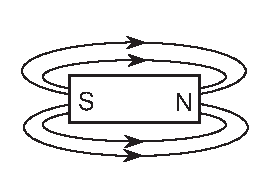
\includegraphics[keepaspectratio,scale=0.66]{Jan2002-Q33-A}}
      \correctchoice{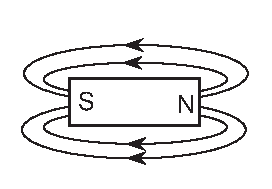
\includegraphics[keepaspectratio,scale=0.66]{Jan2002-Q33-B}}
        \wrongchoice{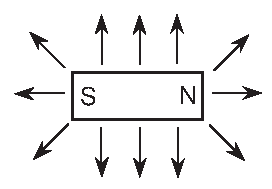
\includegraphics[keepaspectratio,scale=0.66]{Jan2002-Q33-C}}
        \wrongchoice{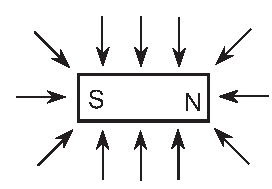
\includegraphics[keepaspectratio,scale=0.66]{Jan2002-Q33-D}}
    \end{choices}
    \end{multicols}
\end{question}
}


%% Section June2001
%%--------------------
\element{nysed}{
\begin{question}{June2001-Q34}
    The diagram below represents the magnetic lines of force around a bar magnet.
    \begin{center}
    \begin{tikzpicture}
        \begin{scope}[decoration={markings,mark=at position 0.5 with {\arrow{latex}}}]
            \clip (-4,-3) rectangle (4,3);
            %% field lines
            %% NOTE: make controls points not inline with point??
            \foreach \x/\y in {20/8,40/4,60/2} {
                \draw[thick,postaction={decorate}] (-1.7,0) .. controls ++({180-\x}:\y) and ++({360+\x}:\y) .. (1.7,0);
                \draw[thick,postaction={decorate}] (-1.7,0) .. controls ++({180+\x}:\y) and ++({360-\x}:\y) .. (1.7,0);
            }
            %% magnet
            \draw[fill=white] (-2,-0.5) rectangle (+2,+0.5);
            \node[anchor=west] at (-2,0) {N};
            \node[anchor=east] at (+2,0) {S};
            %% options
            \fill (-2.5,0) circle (1.5pt) node[anchor=east] {$A$};
            \fill (-3,1.5) circle (1.5pt) node[anchor=south east] {$B$};
            \fill (0,2) circle (1.5pt) node[anchor=south] {$C$};
            \fill (0,1) circle (1.5pt) node[anchor=south] {$D$};
        \end{scope}
    \end{tikzpicture}
    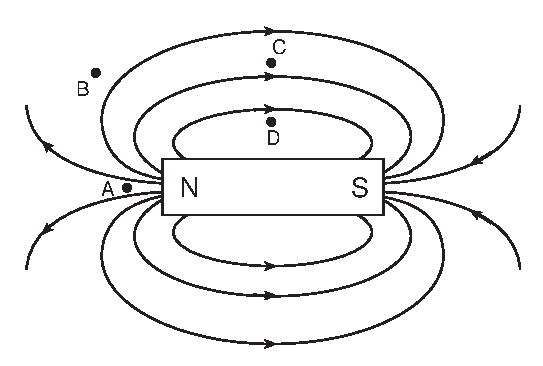
\includegraphics[keepaspectratio,scale=0.75]{June2001-Q34}
    \end{center}
    At which point is the magnitude of the magnetic field strength of the bar magnet the greatest?
    \begin{multicols}{4}
    \begin{choices}[o]
      \correctchoice{$A$}
        \wrongchoice{$B$}
        \wrongchoice{$C$}
        \wrongchoice{$D$}
    \end{choices}
    \end{multicols}
\end{question}
}

\element{nysed}{
\begin{question}{June2001-Q35}
    The diagram below shows an electromagnet made from a nail,
        a coil of insulated wire, and a battery.
    \begin{center}
        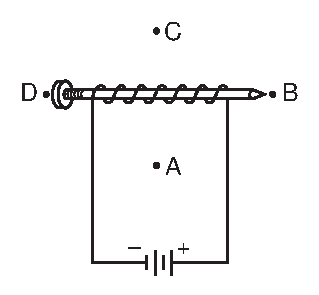
\includegraphics[keepaspectratio,scale=0.75]{June2001-Q35}
    \end{center}
    The south pole of the electromagnet is located closest to point:
    \begin{multicols}{4}
    \begin{choices}[o]
        %% NOTE: positive terminal conventional current
        \wrongchoice{$A$}
        \wrongchoice{$B$}
        \wrongchoice{$C$}
      \correctchoice{$D$}
    \end{choices}
    \end{multicols}
\end{question}
}

%% Section Jan2001
%%--------------------
\element{nysed}{
\begin{question}{Jan2001-Q34}
    In the diagram below, a wire carrying an electron current into the page,
        as denoted by $X$, is placed in a magnetic field.
    \begin{center}
        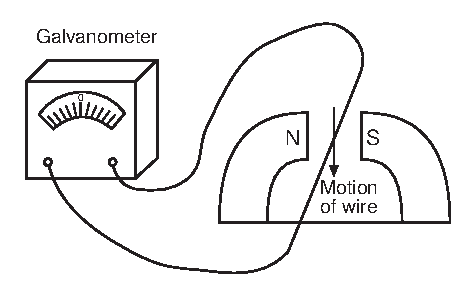
\includegraphics[keepaspectratio,scale=0.75]{June2001-Q78}
    \end{center}
    The magnetic field exerts a force on the wire toward point:
    \begin{multicols}{4}
    \begin{choices}
      \correctchoice{$A$}
        \wrongchoice{$B$}
        \wrongchoice{$C$}
        \wrongchoice{$D$}
    \end{choices}
    \end{multicols}
\end{question}
}

\element{nysed}{
\begin{question}{Jan2001-Q37}
    A wire conductor is moved at constant speed perpendicularly to a uniform magnetic field.
    If the strength of the magnetic field is increased,
        the induced potential across the ends of the conductor:
    \begin{choices}
        \wrongchoice{decreases}
      \correctchoice{increases}
        \wrongchoice{remains the same}
    \end{choices}
\end{question}
}


%% Section June2000
%%--------------------
\element{nysed}{
\begin{question}{June2000-Q31}
    Which diagram best represents the magnetic field around a straight wire in which electrons are flowing from left to right?
    %% NOTE: TODO: double check current!!
    \begin{multicols}{2}
    \begin{choices}
        \AMCboxDimensions{down=-11mm}
        \correctchoice{
            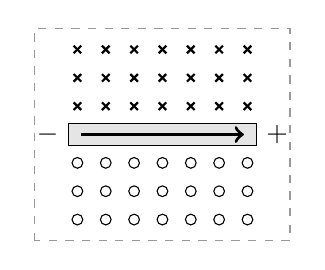
\begin{tikzpicture}[scale=0.9]
                \draw[dashed,white!60!black] (-1.8,-1.5) rectangle (1.8,1.5);
                %% wire
                \draw[fill=white!90!black] (-1.33,-0.15) rectangle (1.33,0.15);
                \node[anchor=east] at (-1.33,0) {$-$};
                \node[anchor=west] at (+1.33,0) {$+$};
                \draw[very thick,->] (-1.15,0) -- (1.15,0);
                %% field lines
                \foreach \x in {-12,-8,-4,0,4,8,12} {
                    \foreach \y in {4,8,12}
                        \foreach \z in {45,135,225,315}
                            \draw[thick] (\x mm,\y mm) -- ++(\z:0.5ex);
                    \foreach \y in {-4,-8,-12}
                        \draw (\x mm,\y mm) circle (0.5ex);
                }
            \end{tikzpicture}
        }
        \wrongchoice{
            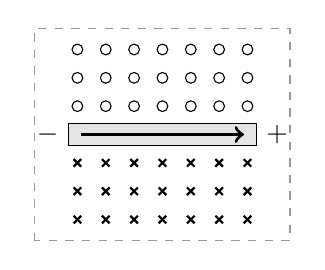
\begin{tikzpicture}[scale=0.9]
                \draw[dashed,white!60!black] (-1.8,-1.5) rectangle (1.8,1.5);
                %% wire
                \draw[fill=white!90!black] (-1.33,-0.15) rectangle (1.33,0.15);
                \node[anchor=east] at (-1.33,0) {$-$};
                \node[anchor=west] at (+1.33,0) {$+$};
                \draw[very thick,->] (-1.15,0) -- (1.15,0);
                %% field lines
                \foreach \x in {-12,-8,-4,0,4,8,12} {
                    \foreach \y in {4,8,12}
                        \draw (\x mm,\y mm) circle (0.5ex);
                    \foreach \y in {-4,-8,-12}
                        \foreach \z in {45,135,225,315}
                            \draw[thick] (\x mm,\y mm) -- ++(\z:0.5ex);
                }
            \end{tikzpicture}
        }
        \wrongchoice{
            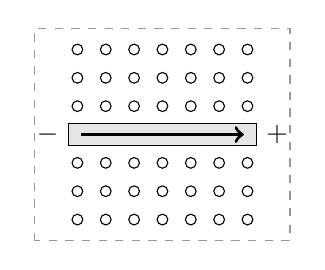
\begin{tikzpicture}[scale=0.9]
                \draw[dashed,white!60!black] (-1.8,-1.5) rectangle (1.8,1.5);
                %% wire
                \draw[fill=white!90!black] (-1.33,-0.15) rectangle (1.33,0.15);
                \node[anchor=east] at (-1.33,0) {$-$};
                \node[anchor=west] at (+1.33,0) {$+$};
                \draw[very thick,->] (-1.15,0) -- (1.15,0);
                %% field lines
                \foreach \x in {-12,-8,-4,0,4,8,12} {
                    \foreach \y in {-12,-8,-4,4,8,12}
                        \draw (\x mm,\y mm) circle (0.5ex);
                }
            \end{tikzpicture}
        }
        \wrongchoice{
            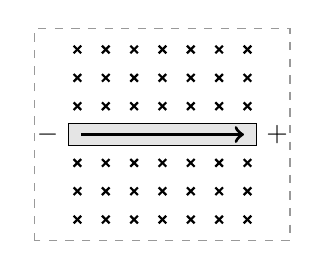
\begin{tikzpicture}[scale=0.9]
                \draw[dashed,white!60!black] (-1.8,-1.5) rectangle (1.8,1.5);
                %% wire
                \draw[fill=white!90!black] (-1.33,-0.15) rectangle (1.33,0.15);
                \node[anchor=east] at (-1.33,0) {$-$};
                \node[anchor=west] at (+1.33,0) {$+$};
                \draw[very thick,->] (-1.15,0) -- (1.15,0);
                %% field lines
                \foreach \x in {-12,-8,-4,0,4,8,12} {
                    \foreach \y in {-12,-8,-4,4,8,12}
                        \foreach \z in {45,135,225,315}
                            \draw[thick] (\x mm,\y mm) -- ++(\z:0.5ex);
                }
            \end{tikzpicture}
        }
    \end{choices}
    \end{multicols}
\end{question}
}

\element{nysed}{
\begin{question}{June2000-Q38}
    The diagram below shows an electron, $e$,
        located in a magnetic field
    \begin{center}
        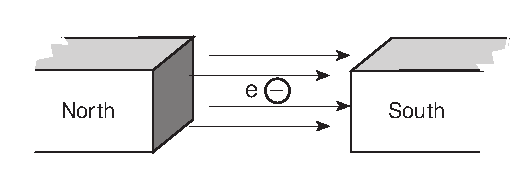
\includegraphics[keepaspectratio,scale=0.75]{June2000-Q38}
    \end{center}
    There is no magnetic force on the electron when it moves
    \begin{choices}
      \correctchoice{toward the right side of the page}
        \wrongchoice{toward the top of the page}
        \wrongchoice{into the page}
        \wrongchoice{out of the page}
    \end{choices}
\end{question}
}

%% Section June1999
%%--------------------


%% Section June1998
%%--------------------

%% NOTE: June1998-Q33: possible duplicate of graphic
%% NOTE: June1998-Q36: needs graphic

\element{nysed}{
\begin{question}{June2000-Q34}
    Two bar magnets of equal strength are positioned as shown.
    \begin{center}
    \begin{tikzpicture}
        %% labels
        \fill (0,0) circle (1.5pt) node[anchor=north] {$B$};
        \fill (1,-1) circle (1.5pt) node[anchor=north] {$A$};
        \fill (3.5,0) circle (1.5pt) node[anchor=north] {$D$};
        \fill (2,1) circle (1.5pt) node[anchor=north] {$C$};
        %% left magnet
        \node[anchor=center,draw,minimum width=2cm,minimum height=2em] (A) at (-2,0) {};
        \node[anchor=west] at (A.west) {S};
        \node[anchor=east] at (A.east) {N};
        %% right magnet
        \node[anchor=center,draw,minimum width=2cm,minimum height=2em] (B) at (2,0) {};
        \node[anchor=west] at (B.west) {S};
        \node[anchor=east] at (B.east) {N};
    \end{tikzpicture}
    \end{center}
    At which point is the magnetic flux density due to the two magnets greatest?
    \begin{multicols}{4}
    \begin{choices}[o]
        \wrongchoice{$A$}
      \correctchoice{$B$}
        \wrongchoice{$C$}
        \wrongchoice{$D$}
    \end{choices}
    \end{multicols}
\end{question}
}

\element{nysed}{
\begin{question}{June2000-Q38}
    The diagram below shows an electron, $e$,
        located in a magnetic field
    \begin{center}
        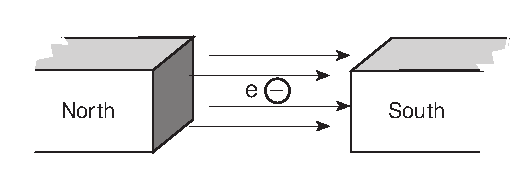
\includegraphics[keepaspectratio,scale=0.75]{June2000-Q38}
    \end{center}
    There is no magnetic force on the electron when it moves
    \begin{choices}
      \correctchoice{toward the right side of the page}
        \wrongchoice{toward the top of the page}
        \wrongchoice{into the page}
        \wrongchoice{out of the page}
    \end{choices}
\end{question}
}


%% Section June1997
%%--------------------

%% NOTE: June1997-Q33 tikz?
%% NOTE: June1997-Q34 requires graphic
%% NOTE: June1997-Q35 tikz?


%% Section June1996
%%--------------------
%\element{nysed}{
%\begin{question}{June1996-Q33}
%    The diagram below shows an electron current in
%        a wire loop.
%    \begin{center}
%        %% NOTE: include tikz
%    \end{center}
%    What is the direction of the magnetic field at the
%        center of the loop?
%    \begin{choices}
%      \correctchoice{out of the page}
%        \wrongchoice{into the page}
%        \wrongchoice{clockwise}
%        \wrongchoice{counterclockwise}
%    \end{choices}
%\end{question}
%}

\element{nysed}{
\begin{question}{June1996-Q34}
    A charged particle is moving with a constant velocity.
    On entering a uniform magnetic field,
        the particle
    \begin{choices}
        \wrongchoice{must decrease in speed}
        \wrongchoice{must change the magnitude of its momentum}
      \correctchoice{may change its direction of motion}
        \wrongchoice{may increase in kinetic energy}
    \end{choices}
\end{question}
}

%\element{nysed}{
%\begin{question}{June1996-Q37}
%    Which diagram correctly shows a magnetic field configuration?
%    \begin{multicols}{2}
%    \begin{choices}
%        %% NOTE: add graphics
%        \wrongchoice{}
%    \end{choices}
%    \end{multicols}
%\end{question}
%}


%% Section June1994
%%--------------------
\element{nysed}{
\begin{question}{June1994-Q32}
    Electrons are flowing in a conductor as shown in the diagram.
    \begin{center}
    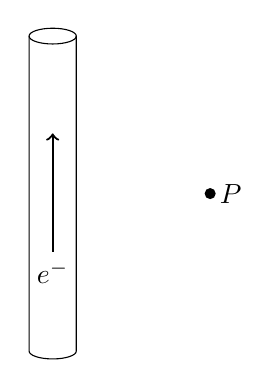
\begin{tikzpicture}
        %% electron flow
        \draw (-0.3,2) -- (-0.3,-2) arc(180:360:0.3 and 0.1) to (0.3,2) arc(0:180:0.3 and 0.1);
        \draw (0.3,2) arc(360:180:0.3 and 0.1);
        \node[anchor=center] (E) at (0,-1) {$e^-$};
        \draw[thick,->] (E.north) -- ++(90:1.5);
        %% point P
        \fill (2,0) circle (2pt) node[anchor=west] {$P$};
    \end{tikzpicture}
    \end{center}
    What is the direction of the magnetic field at point $P$?
    \begin{choices}
        \wrongchoice{toward the top of the page}
        \wrongchoice{toward the bottom of the page}
        \wrongchoice{into the page}
      \correctchoice{out of the page}
    \end{choices}
\end{question}
}

\element{nysed}{
\begin{question}{June1994-Q35}
    An electron moving in a uniform magnetic field experiences the maximum magnetic force when the angle between the direction of the electron's motion and the direction of the magnetic field is:
    \begin{multicols}{4}
    \begin{choices}
        \wrongchoice{\ang{0}}
        \wrongchoice{\ang{45}}
      \correctchoice{\ang{90}}
        \wrongchoice{\ang{180}}
    \end{choices}
    \end{multicols}
\end{question}
}


%% Section June1986
%%--------------------
\element{nysed}{
\begin{question}{June1986-Q45}
    A magnetic force is experienced by an electron moving through a magnetic field.
    If the electron were replaced by a proton traveling at the same velocity,
        the magnitude of the magnetic force experienced by the proton would be:
    \begin{multicols}{2}
    \begin{choices}
      \correctchoice{the same}
        \wrongchoice{twice as great}
        \wrongchoice{half as great}
        \wrongchoice{zero}
    \end{choices}
    \end{multicols}
\end{question}
}

\element{nysed}{
\begin{question}{June1986-Q60}
    A wire conductor moves perpendicularly at constant speed through a magnetic field.
    If the flux density increases,
        the potential difference induced across the ends of the wire will:
    \begin{choices}
        \wrongchoice{decrease}
      \correctchoice{increase}
        \wrongchoice{remain the same}
    \end{choices}
\end{question}
}


%% Section June1985
%%--------------------
\element{nysed}{
\begin{question}{June1985-Q46}
    The magnitude of the electric potential induced across the ends of a conductor moving in a magnetic field may be increased by:
    \begin{choices}
        \wrongchoice{increasing the diameter of the conductor}
      \correctchoice{increasing the speed of the conductor}
        \wrongchoice{decreasing the resistance of the conductor}
        \wrongchoice{decreasing the length of the conductor}
    \end{choices}
\end{question}
}



\endinput


